\sepframe{IV. End-to-end\\Differentiable Relaxations}
\begin{frame}[plain]%
\frametitle{End-to-end differentiable relaxations}
\begin{enumerate}
\item Digging into softmax
\item Alternatives to softmax
\item Generalizing to structured prediction
\item Stochasticity and global structures
\end{enumerate}
\end{frame}

\begin{frame}%
\frametitle{%
\alt<1>{Recall: Discrete choices \& differentiability}{One solution: smooth
relaxation}}
\centering
%
\def\vecwidth{.8}
\def\vecheight{.8}
\tikzset{elem/.style={ultra thick,mybg}}
%
\begin{tikzpicture}%
%
\node[anchor=south] at (-1-.5*\vecwidth, \vecheight*5+.1) {$\s$};

\drawcs
\drawscores
\onslide<1>{\drawargmax[\z]}
\onslide<2->{\drawsoftmax[\p]}

\draw[elem,fill=vecfg!50!vecbg] (-1-\vecwidth, \vecheight*4) rectangle (-1, \vecheight*5);
%\node[anchor=south] at (1+.5*\vecwidth, \vecheight*5+.1) {$\hat{\p}$};
\draw[elem,fill=vecbg]  (1, \vecheight*4) rectangle (1+\vecwidth, \vecheight*5);
\draw[elem,fill=vecfg!70!vecbg] (1, \vecheight*3) rectangle (1+\vecwidth, \vecheight*4);

\onslide<3>{\node at (1+.5*\vecwidth, \vecheight*2) {\emoji{frown}};}

\node[anchor=south,align=center] at (-6, \vecheight*3+1) (in) {\phantom{input}};
\node[anchor=south,align=center] at (6, \vecheight*3+1) (out) {\phantom{output}};
%
\node at (0, -1) {$\frac{\partial \alt<1>{\z}{\p}}{\partial \s}=$
\alt<1>{$\bs{0}$ {\small or n/a}}{\emoji{happ}}};
\node[anchor=south,align=center] at (-6, \vecheight*3+1) (in) {input\\$\bs{x}$};
\node[anchor=south] at (-2, \vecheight*3+1) (in-end) {};
\node[anchor=south,align=center] at (6, \vecheight*3+1) (out){output\\$\widehat{\bs{y}}$};
\node[anchor=south] at (2, \vecheight*3+1) (out-end) {};
%
\path (in) edge[->,very thick,bend right=50] node[anchor=north] (ff) {$\s =
    %\bs{f}_1(\bs{x};\bs{w})$} (in-end);
    \bs{f}_{\parp}(\bs{x})$} (in-end);
\path (out-end) edge[->,very thick,bend right=50] node[anchor=north] {$y =
    %f_2(\alt<1>{\z}{\p}, \bs{x}; \bs{w})$} (out);
    \bs{g}_{\clfp}(\z, \bs{x})$} (out);
\node at (0, -2) {\alt<1>{(argmax)}{(softmax)}};
\node<2->[font={\fontsize{10pt}{10}\selectfont},below=50pt of
ff,anchor=north,align=center] {%
$\p = \softmax(\s) = \EE[\z]$, i.e.\\
replace $\EE\big[f(\z)\big]$ with $f\big(\EE[\z]\big)$
};
\end{tikzpicture}
\\[6ex]
\begin{tikzpicture}[overlay]
    \draw[axisline,->] (3, 3) -- (3, 5.5) node[left] {$\pp_1$};
    \draw[axisline,->] (3, 3) -- (7, 3) node[right]{$\ss_1$};

    \node[axislabel,left] at (3, 3) {$0$};
    \node[axislabel,left] at (3, 5) {$1$};

    \draw[axisline] ($(3,3) + (-\ticksize, 0)$) -- ($(3,3) + (+\ticksize, 0)$);
    \draw[axisline] ($(3,4) + (-\ticksize, 0)$) -- ($(3,4) + (+\ticksize, 0)$);
    \draw[axisline] ($(3,5) + (-\ticksize, 0)$) -- ($(3,5) + (+\ticksize, 0)$);

    \draw[axisline] ($(3,3) + (0, -\ticksize)$) -- ($(3,3) + (0, +\ticksize)$);
    \draw[axisline] ($(4,3) + (0, -\ticksize)$) -- ($(4,3) + (0, +\ticksize)$);
    \draw[axisline] ($(5,3) + (0, -\ticksize)$) -- ($(5,3) + (0, +\ticksize)$);
    \draw[axisline] ($(6,3) + (0, -\ticksize)$) -- ($(6,3) + (0, +\ticksize)$);

    \node[axislabel,below] at (4, 3) {$\ss_2 - 1$};
    \node[axislabel,below] at (5, 3) {$\ss_2$};
    \node[axislabel,below] at (6, 3) {$\ss_2 + 1$};

    \draw[ultra thick,colorArgmax] (3, 3) -- (5,3) ;
    \draw[ultra thick,colorArgmax] (5, 5) -- (7,5) ;

\onslide<2->{%
    \draw (3, 3.1) edge[colorSoftmax,ultra thick,out=360,in=180,looseness=1.5] (7, 4.9);
}
\end{tikzpicture}%
\end{frame}

\againframe<3>{overview}

\begin{frame}[t,fragile]%
\frametitle{What is softmax?}%
\centering \fontsize{12pt}{15}\selectfont
Often defined via $\displaystyle
{\pp}_i = \frac{\exp \ss_i}{\sum_j \exp \ss_j}$,\quad
but where does it come from?% \\[1ex]
\begin{columns}
\begin{column}{.62\textwidth}
\centering
\begin{itemize}
\item<2->[] $\p \in \simplex$: probability distribution over choices
\item<6->[] Expected score under $\p$: $\EE_{i \sim \p}~\ss_i =\p^\top\s$
\item<7->[] \textbf{argmax} \onslide<8->{maximizes \textbf{expected score}}
\item<9->[] Shannon entropy of $\p$: $\HH(\p) = -\sum_i \pp_i \log \pp_i$
\item<10->[] \textbf{softmax} maximizes \textbf{expected score} $+$ \textbf{entropy}:
\end{itemize}
\end{column}%
\begin{column}{.33\textwidth}
\begin{overlayarea}{\textwidth}{6\baselineskip}
\centering
\only<9>{%
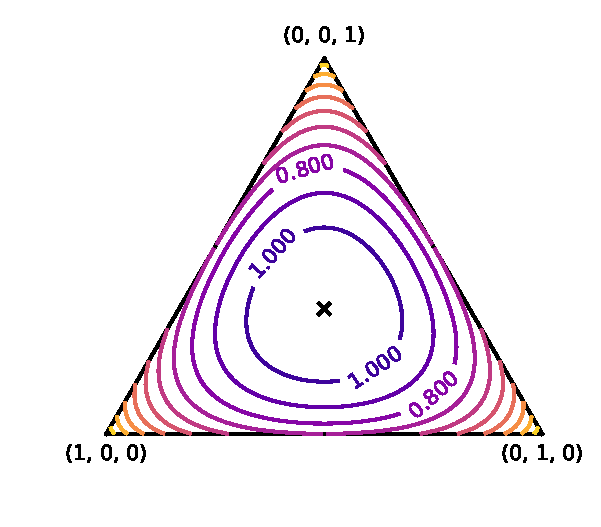
\includegraphics[width=.99\textwidth]{img/4011_simplex_0_softmax.pdf}
}%
\only<10>{%
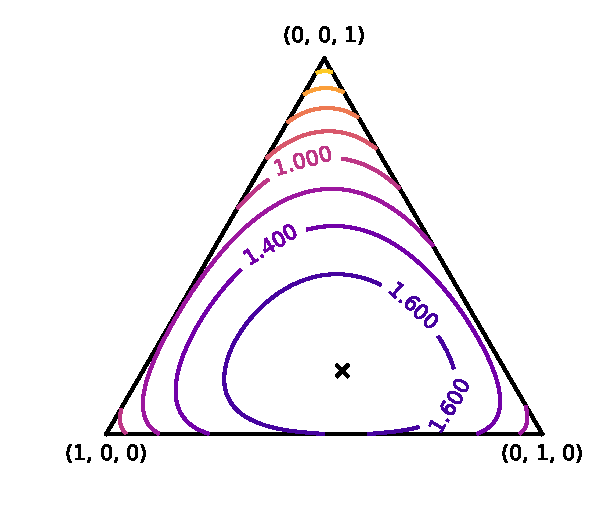
\includegraphics[width=.99\textwidth]{img/4011_simplex_1_softmax.pdf}\\
$\displaystyle \argmax_{\p \in \simplex} \p^\top\s + \HH(\p)$
}%
\onslide<2-8>{%
\begin{tikzpicture}[every node/.style={inner sep=0,outer sep=2pt}]
    \begin{axis}[
        small,
        xmin=-.1, xmax=1.5,
        ymin=-.1, ymax=1.5,
        zmin=-.1, zmax=1.5,
        height=6cm,
        width=8cm,
        xtick={0, .5, 1, 1.5},
        ytick={.5, 1, 1.5},
        ztick={.5, 1, 1.5},
        axis line style=thick,
        axis lines=middle,
        axis equal,
        compat=1.6,
        view={60}{15}
        ]

    \node at (axis cs:1, 0, 0) (A) {};
    \node at (axis cs:0, 1, 0) (B) {};
    \node at (axis cs:0, 0, 1) (C) {};

    \only<2->{%
    \addplot3[color=tDY,ultra thick,fill=tDY,fill opacity=.5] coordinates { (0,0,1) (0,1,0) (1,0,0) (0,0,1) };

    \draw[tBleu,fill] (A) circle[radius=2pt];
    \draw[tBleu,fill] (B) circle[radius=2pt];
    \draw[tBleu,fill] (C) circle[radius=2pt];
    }

    \def\ofst{.3,.3,.4}
    \only<3>{%
    \node[anchor=south west,font=\small]
        at ($(B) + .5*(axis direction cs:\ofst)$)
        (lblB) {$\p = [0, 1, 0]$};
    \draw[thick,fg,->] (lblB.south west) -- (B);
    }

    \only<4>{%
    \node[anchor=south west,font=\small]
        at ($(C) + (axis direction cs:\ofst)$)
        (lblC) {$\p = [0, 0, 1]$};
    \draw[thick,fg,->] (lblC.south west) -- (C);
    }

    \only<5>{%
    \node at (axis cs:.33,.33,.33) (mid) {};
    \draw[tBleu,fill] (mid) circle[radius=2pt];
    \node[anchor=south west,font=\small]
        at ($(mid) + (axis direction cs:\ofst)$)
        (lblmid) {$\p = \left[\nicefrac{1}{3}, \nicefrac{1}{3},
    \nicefrac{1}{3}\right]$};
    \draw[thick,fg,->] (lblmid.south west) -- (mid);
    }

    \only<6->{%
        \node[anchor=west,label=east:{\small $\s=[.7, .1, 1.5]$}] at
        (axis cs:.7,.1,1.5) (s) {};
        \draw[tVividBlue,fill] (s) circle[radius=2pt];
    }
    \only<6->{%
        % We cannot use foreach inside pgfplots axis environment.
        % also, we need fragile AND double the ##
        \pgfplotsinvokeforeach{90,80,...,10}{
            \draw[ultra thick,tPeony!##1!tTarmac]
            %(axis cs: .05+1-.01*##1,0,-.05+.01*##1)  % slignt .05 skew
            (axis cs: 1-.01*##1,0,.01*##1)  % slignt .05 skew
            -- (axis cs: 0,1-.01*##1,.01*##1);
        }
    }
    \only<8->{
        \node[anchor=south west,font=\small]
            at ($(C) + (axis direction cs:.3,.3,-.1)$)
            (lblCstar) {$\p^\star = [0, 0, 1]$};
        \draw[thick,fg,->] (lblCstar.west) -- (C);
        \draw[colorArgmax,fill] (C) circle[radius=3pt];
    }

    \end{axis}
\end{tikzpicture}}%
\\
\only<8->{%
$\displaystyle \argmax_{\p \in \simplex} \p^\top\s$
\\[1ex]
}
\end{overlayarea}
\end{column}
\end{columns}
\end{frame}

\begin{frame}[t]
\frametitle{Variational form of softmax}
\small
\setlength{\abovedisplayskip}{5pt}%
\setlength{\belowdisplayskip}{5pt}%
\setlength{\abovedisplayshortskip}{0pt}%
\setlength{\belowdisplayshortskip}{0pt}
\centering
\textbf{Proposition.} The unique solution to~~
$\displaystyle \argmax_{\p \in \simplex} \p^\top\s + \HH(\p)$
~~is given by $\pp_j = \frac{\exp \ss_j}{\sum_i \exp \ss_i}$.
\\[\baselineskip]
\begin{columns}[t]
\begin{column}{.49\textwidth}
\uncover<2->{%
Explicit form of the optimization problem:
\begin{align*}
\text{maximize}\quad&\textstyle \sum_j \pp_j \ss_j - \pp_j \log \pp_j \\
\text{subject to}\quad& \p \geq 0,~\p^\top \bs{1} = 1
\end{align*}}
\uncover<3->{%
Lagrangian:
$$\mathcal{L}(\p, \bs{\nu}, \tau) = \textstyle -\sum_j \pp_j \ss_j - \pp_j \log \pp_j - \p^\top\bs{\nu} + \tau(\p^\top\bs{1} - 1)$$}
\uncover<4->{%
Optimality conditions (KKT):
\begin{align*}
0 &= \nabla_{p_i} \mathcal{L}(\p, \bs{\nu}, \tau) = -\ss_i + \log \pp_i + 1 - \nu_i +
\tau
\\
\p^\top\bs{\nu} &= 0 \\
\p &\in \triangle \\
\bs{\nu} &\geq \bs{0} \\
\end{align*}}
\end{column}
\begin{column}{.45\textwidth}
\uncover<5->{$\log \pp_i = \ss_i + \nu_i - (\tau + 1)$}\\
\uncover<6->{\quad if $\pp_i = 0$, r.h.s.\ must be $-\infty$,\\
\quad thus $\pp_i > 0$, so $\nu_i = 0$.\\[1ex]}
\uncover<7->{$\pp_i = \nicefrac{\exp(\ss_i)}{\exp(\tau + 1)} =
\nicefrac{\exp(\ss_i)}{Z}$\\[1ex]}
\uncover<8->{Must find $Z$ such that $\sum_j \pp_j = 1$. \\}
\uncover<9->{Answer:  $Z = \sum_j \exp(\ss_j)$ \\[1ex]}
\uncover<10->{So, $\displaystyle \pp_i = \frac{\exp(\ss_i)}{\sum_j \exp(\ss_j)}$. \\[3ex]
\textcolor{mygr}{Classic result, e.g., \citep{boyd,Wainwright2008}}}
\end{column}
\end{columns}
\end{frame}


\begin{frame}[t]
\frametitle{Generalizing softmax: Smoothed argmaxes}
\vspace{-.5\baselineskip}
\begin{columns}[T]
\begin{column}{.58\textwidth}
\centering
$\displaystyle \mapo(\s) = \argmax_{\p \in \simplex} \p^\top\s - \Omega(\p)$
\fontsize{12.5pt}{13}\selectfont%
\\
%{
\def\vph{\vphantom{$\sum_j$}}
\renewcommand{\arraystretch}{1.7}
\begin{tabular}{r@{~}r@{:~~}r@{$\,=\,$}l}
\onslide<3->{
\colorbul{colorArgmax} &
argmax    & $\Omega(\p)$ & \vph $0$ \\}
\onslide<4->{
\colorbul{colorSoftmax} &
softmax   & $\Omega(\p)$ & $\sum_j \pp_j \log \pp_j$ \\}
\onslide<5->{
\colorbul{colorSparsemax} &
sparsemax & $\Omega(\p)$ & \vph $\nicefrac{1}{2} \|\p\|^2_2$ \\}
\onslide<6->{
%\multicolumn{4}{l}{\footnotesize Generalized entropy in between:}\\
&$\alpha$-entmax  & $\Omega(\p)$ & \vph
    $\nicefrac{1}{\alpha(\alpha-1)} \sum_j \pp_i^\alpha$\\%
}
\only<7->{
%\colorbul{colorFusedmax} &
&
fusedmax  & $\Omega(\p)$ & \vph
    $\nicefrac{1}{2} \|\p\|^2_2 + \sum_j |\pp_j -\pp_{j-1}|$\\%
%\colorbul{colorFusedmax} &
&
csparsemax  & $\Omega(\p)$ & \vph
    $\nicefrac{1}{2} \|\p\|^2_2 + \iota(\bs{a} \leq \p \leq \bs{b})$\\%
&
csoftmax  & $\Omega(\p)$ & \vph
$\sum_j \pp_j \log \pp_j + \iota(\bs{a} \leq \p \leq \bs{b})$\\%
}
\end{tabular}%

\small
\only<6>{Generalized entropy interpolates in between \citep{Tsallis1988}\\
Used in Sparse Seq2Seq: \citep{sparseseq} \\ (Mon 13:50, poster session 2D)}
% Monday, 13:50, poster session 2D
%}%
\end{column}%
%
%
\begin{column}{.30\textwidth}
\centering
% BEGIN softmax 2d plot
\begin{tikzpicture}[baseline=(current bounding box.north),scale=.9]
    \draw[axisline,->] (3, 3) -- (3, 5.5) node[left] {$\pp_1$};
    \draw[axisline,->] (3, 3) -- (7, 3) node[right]{$\ss_1$};

    \node[axislabel,left] at (3, 3) {$0$};
    \node[axislabel,left] at (3, 5) {$1$};

    \draw[axisline] ($(3,3) + (-\ticksize, 0)$) -- ($(3,3) + (+\ticksize, 0)$);
    \draw[axisline] ($(3,4) + (-\ticksize, 0)$) -- ($(3,4) + (+\ticksize, 0)$);
    \draw[axisline] ($(3,5) + (-\ticksize, 0)$) -- ($(3,5) + (+\ticksize, 0)$);

    \draw[axisline] ($(3,3) + (0, -\ticksize)$) -- ($(3,3) + (0, +\ticksize)$);
    \draw[axisline] ($(4,3) + (0, -\ticksize)$) -- ($(4,3) + (0, +\ticksize)$);
    \draw[axisline] ($(5,3) + (0, -\ticksize)$) -- ($(5,3) + (0, +\ticksize)$);
    \draw[axisline] ($(6,3) + (0, -\ticksize)$) -- ($(6,3) + (0, +\ticksize)$);

    \node[axislabel,below] at (4, 3) {$-1$};
    \node[axislabel,below] at (5, 3) {$0$};
    \node[axislabel,below] at (6, 3) {$1$};

    \draw<3->[ultra thick,colorArgmax] (3, 3) -- (5,3) ;
    \draw<3->[ultra thick,colorArgmax] (5, 5) -- (7,5) ;
    \draw<4-> (3, 3.1)
        edge[colorSoftmax,ultra thick,out=360,in=180,looseness=1.5] (7, 4.9);
    \draw<5->[ultra thick,colorSparsemax,dashed]
        (3, 3) -- (4,3) -- (6,5) -- (7, 5) ;
\end{tikzpicture}%
% END softmax 2d plot
%\vspace{-.5cm}%
\\
% BEGIN Simplex barycentric
\begin{tikzpicture}[baseline=(current bounding box.north)]
\setupsimplexbary{}
\coordinate (argmax)    at (barycentric cs:L1=0,L2=0,L3=1);
\coordinate (softmax)   at (barycentric cs:L1=.3,L2=.2,L3=.5);
\coordinate (sparsemax) at (barycentric cs:L1=.3,L2=0,L3=.7);

\uncover<3->{%
\node[label=west:{\small $[0,0,1]$}] at (argmax) {};
\draw[point,fill=colorArgmax] (argmax) circle[radius=5pt];}
\uncover<4->{%
\node[label=south:{\small $[.3,.2,.5]$}] at (softmax) {};
\draw[point,fill=colorSoftmax] (softmax) circle[radius=5pt];}
\uncover<5->{%
\node[label=west:{\small $[.3,0,.7]$}] at (sparsemax) {};
\draw[point,fill=colorSparsemax] (sparsemax) circle[radius=5pt];}
\end{tikzpicture}%
%% END Simplex Barycentric
\end{column}%
\end{columns}%
%
\onslide<1-4>{\cornercite{sparseattn}}
\onslide<5>{\cornercite{sparseattn,sparsemax}}
\onslide<6>{\cornercite{sparseattn,fylosses}}
\onslide<7>{\cornercite{sparseattn,easy,Malaviya2018ACL}}
%\begin{tikzpicture}[font=\footnotesize,remember picture,overlay]
    %\node<6>[anchor=north east] at (current page.north east) {
        %\citep{sparseattn}};
    %\node<5>[anchor=south west] at (current page.south west) {
        %\citep{sparsemax}};
%\end{tikzpicture}
%\onslide<2>{\overlaybox{$\bs{\pi}_{\Omega}$ differentiable when $\Omega$
%strongly convex.}}
\end{frame}%

\againframe<4>{marginalpoly}

% MAIN IDEA
%
\begin{frame}<1-7>[label=mainidea]%
\onslide<8->{\cornercite{sparsemap}}%
\vspace{-\baselineskip}
\begin{columns}[T]%
\begin{column}{.45\textwidth}\centering%
\vbox to .9\textheight{%
{%
\fontsize{12.5pt}{13}\selectfont%
\setlength{\tabcolsep}{2pt}%
\renewcommand{\arraystretch}{2}%
\begin{tabular}{r r l}
\onslide<2->{%
\colorbul{colorArgmax} &
\textbf{argmax} &
$\displaystyle \argmax_{\p \in \triangle} \p ^\top \s$ \\
}
\onslide<4->{%
\colorbul{colorSoftmax} &
\textbf{softmax} &
$\displaystyle \argmax_{\p \in \triangle} \p ^\top \s + \HH(\p)$ \\
}
\onslide<8->{%
\colorbul{colorSparsemax} &
\textbf{sparsemax} &
$\displaystyle \argmax_{\p \in \triangle} \p ^\top \s - \nicefrac{1}{2} \|\p\|^2$
}%
\end{tabular}%
}
\vfill
\begin{tikzpicture}
\setupsimplexbary[2.5]{}
\coordinate (argmax)    at (barycentric cs:L1=0,L2=0,L3=1);
\coordinate (softmax)   at (barycentric cs:L1=.3,L2=.2,L3=.5);
\coordinate (sparsemax) at (barycentric cs:L1=.3,L2=0,L3=.7);

\onslide<2->{
\draw[point,fill=colorArgmax] (argmax) circle[radius=5pt];
}
\onslide<4->{
\draw[point,fill=colorSoftmax] (softmax) circle[radius=5pt];
}
\onslide<8->{
\draw[point,fill=colorSparsemax] (sparsemax) circle[radius=5pt];
}
\end{tikzpicture}}\end{column}
\begin{column}{.54\textwidth}\centering
\vbox to .9\textheight{%
{%
\fontsize{12.5pt}{13}\selectfont%
\setlength{\tabcolsep}{2pt}%
\renewcommand{\arraystretch}{2}%
\begin{tabular}{r l l@{\quad}}
\onslide<3->{%
\textbf{MAP} &
$\displaystyle \argmax_{\mg \in \Mp} \mg ^\top \pr$ &
\colorbul{colorArgmax} \\
}%
\onslide<5->{%
\textbf{marginals} &
$\displaystyle \argmax_{\mg \in \Mp} \mg ^\top \pr + \widetilde{\HH}(\mg)$ &
\colorbul{colorSoftmax} \\
}%
\onslide<9->{%
\textbf{SparseMAP} &
$\displaystyle \argmax_{\mg \in \Mp} \mg ^\top \pr - \nicefrac{1}{2} \|\mg\|^2$ &
\colorbul{colorSparsemax}
}%
\end{tabular}%
}
\vfill
\begin{tikzpicture}[node distance=0pt]%
\uncover<1->{
\node[
    ultra thick,
    draw=colorPolytope,
    fill=colorPolytope,
    fill opacity=.15,
    minimum size=2.5cm,
    regular polygon, regular polygon sides=6] (mp) {};
\node[label=east:{\small$\mathcal{M}$}] at (mp.corner 5) {};
\foreach \i in {1, ..., 6}%
{
    \draw[colorPolytope,fill] (mp.corner \i) circle[radius=3pt];
}
}
\coordinate (L1) at (mp.corner 3);
\coordinate (L2) at (mp.corner 5);
\coordinate (L3) at (mp.corner 2);
\coordinate (argmax)    at (L3);
\coordinate (softmax)   at (barycentric cs:L1=.25,L2=.25,L3=.45);
\coordinate (sparsemax) at (barycentric cs:L1=.4,L3=.6);
\onslide<3->{
    \draw[point,fill=colorArgmax] (argmax) circle[radius=5pt];
    \node[above right=of argmax] {\cartoon[.5]{1/4,2/5}};
}
\onslide<5->{
    \draw[point,fill=colorSoftmax] (softmax) circle[radius=5pt];
    \node[below right=of softmax] {\cartoonDense[.5]{}};
}
\onslide<9->{
    \draw[point,fill=colorSparsemax] (sparsemax) circle[radius=5pt];
    \node[left=of sparsemax] {\cartoonSparse[.5]{}};
}
\end{tikzpicture}}\end{column}
\end{columns}
%
%\begin{tikzpicture}[font=\footnotesize,remember picture,overlay]
    %\node<14>[anchor=north east] at (current page.north east) {
        %\textcolor{mygr}{\citep{sparsemap}}};
%\end{tikzpicture}
%\uncover<2-4>{\overlaybox[.33]{
%$\begin{aligned}
    %\Mp &\defeq \conv \big\{ \bs{a}_y : y \in \mathcal{Y} \big\} \\
    %\uncover<3-4>{&= \big\{ \bs{A}\p : \p \in \triangle \big\}} \\
    %\uncover<4>{&= \big\{ \EE_{Y\sim\p}~\bs{a}_Y : \p \in \triangle \big\}}
%\end{aligned}$
%}}
\uncover<6-7>{\overlaybox[.5]{%
    Just like softmax relaxes argmax,\\ marginals relax MAP
\textbf{differentiably}!}}
\uncover<7-7>{\overlaybox[.7]{%
Unlike argmax/softmax, computation is not obvious!}}
\end{frame}

\againframe<2->{algos}

\begin{frame}[t]
\frametitle{Derivatives of marginals 1: DP}
\centering
\begin{itemize}
\item[]<1-> \textbf{Dynamic programming:} marginals by \textbf{Forward-Backward},
\textbf{Inside-Outside}, etc.
\begin{itemize}
\item<3->
Alg. consists of differentiable ops:
PyTorch autograd can handle it! (v. bad idea)
\item<4-> Better book-keeping: \citet{Li2009}, \citet{arthurdp}
\item<5-> With circular dependencies, this breaks! Can get an approximation \citet{ves}
\end{itemize}
\end{itemize}
\vspace{-.5\baselineskip}
\uncover<2->{%
\begin{minipage}{.55\textwidth}
\begin{algorithm}[H]
\caption*{Marginals in a sequence tagging model.}
\setstretch{1.3}
\fontsize{9pt}{9}\selectfont
\begin{algorithmic}[1]
\State input:  $d$ tags, $n$ tokens,
                $\pr_U \in \reals^{n \times d},
                 \pr_V \in \reals^{d \times d}$
\State initialize $\bs{\alpha}_1 = \bs{0}, \bs{\beta}_n = \bs{0}$
\For{$i \in 2, \dots, n$}
\Comment{forward log-probabilities}
%\State $\alpha_{i,k} = (\pr_U)_{i,k} + \log \sum_{k'} \exp
%\big(
%\alpha_{i-1, k'} + (\pr_V)_{k', k}
%\big)
    \State $\alpha_{i,k} = \log \sum_{k'} \exp
\big(
\alpha_{i-1, k'} +
(\pr_U)_{i, k} +
(\pr_V)_{k', k}
\big)$
\hfill for all $k$
\EndFor

\For{$i \in n-1, \dots, 1$}
\Comment{backward log-probabilities}
\State $\beta_{i,k} = \log \sum_{k'} \exp
\big(
\beta_{i+1, k'} + (\pr_U)_{i+1, k'} + (\pr_V)_{k, k'}
\big)$
\hfill for all $k$
\EndFor
\State $Z = \sum_k \exp  \alpha_{n,k}$
\Comment{partition function}
\State \Return $\mg = \exp \big(\bs{\alpha} + \bs{\beta} - \log Z\big)$
\Comment{marginals}
\end{algorithmic}
\end{algorithm}%
\end{minipage}%
\hspace{10pt}%
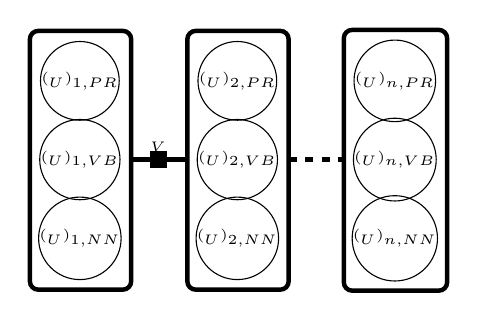
\begin{tikzpicture}[
    baseline=(current bounding box.center),
    font=\tiny,inner sep=0,outer sep=0,
    factoredge/.style={ultra thick},
    factor/.style={fill, rectangle, minimum width=6pt, minimum height=6pt}
]
\node[circle,draw] at (0, 0) (var13) {$(\pr_U)_{1,\text{NN}}$};
\node[circle,draw] at (0, 1) (var12) {$(\pr_U)_{1,\text{VB}}$};
\node[circle,draw] at (0, 2) (var11) {$(\pr_U)_{1,\text{PR}}$};
\coordinate (var1 nw) at ([xshift=-8pt, yshift=8pt] var11.north west);
\coordinate (var1 se) at ([xshift=8pt, yshift=-8pt] var13.south east);
\coordinate (var1 e) at ([xshift=4pt] var12.east);
\draw[rounded corners=3pt, ultra thick] (var1 nw) rectangle (var1 se);

\node[circle,draw] at (2, 0) (var23) {$(\pr_U)_{2,\text{NN}}$};
\node[circle,draw] at (2, 1) (var22) {$(\pr_U)_{2,\text{VB}}$};
\node[circle,draw] at (2, 2) (var21) {$(\pr_U)_{2,\text{PR}}$};
\coordinate (var2 nw) at ([xshift=-8pt, yshift=8pt] var21.north west);
\coordinate (var2 se) at ([xshift=8pt, yshift=-8pt] var23.south east);
\coordinate (var2 w) at ([xshift=-4pt] var22.west);
\coordinate (var2 e) at ([xshift=4pt] var22.east);
\draw[rounded corners=3pt, ultra thick] (var2 nw) rectangle (var2 se);
\path (var1 e) edge[factoredge] node[factor,label=$\pr_V$] {} (var2 w);

\node[circle,draw] at (4, 0) (var33) {$(\pr_U)_{n,\text{NN}}$};
\node[circle,draw] at (4, 1) (var32) {$(\pr_U)_{n,\text{VB}}$};
\node[circle,draw] at (4, 2) (var31) {$(\pr_U)_{n,\text{PR}}$};
\coordinate (var3 nw) at ([xshift=-8pt, yshift=8pt] var31.north west);
\coordinate (var3 se) at ([xshift=8pt, yshift=-8pt] var33.south east);
\coordinate (var3 w) at ([xshift=-4pt] var32.west);
\draw[rounded corners=3pt, ultra thick] (var3 nw) rectangle (var3 se);
\path (var2 e) edge[factoredge,dashed] (var3 w);
\end{tikzpicture}
}%
\end{frame}
\begin{frame}[t]
\frametitle{Derivatives of marginals 2: Matrix-Tree}
\centering
$\bs{L}(\s)$: Laplacian of the edge score graph

\begin{align*}
Z &= \det \bs{L}(\s) \\
\mg &= \bs{L}(\s)^{-1}\\
\nabla \mg &= \nabla \bs{L}^{-1} = \bs{L}^{-1}\left(\pfrac{\bs{L}}{\pr}\right) \bs{L}^{-1} \\
\end{align*}%
\end{frame}

\begin{frame}[t]
\frametitle{Structured Attention Networks}
\def\vecwidth{.8}
\def\vecheight{.8}
\centering
\begin{tikzpicture}[
    outer sep=0,
    factoredge/.style={ultra thick},
    factor/.style={inner sep=0,font=\tiny,fill, rectangle, minimum width=6pt, minimum height=6pt}
]
\node<1>[font=\small,anchor=south] at (0, \vecheight*4) {la};
\node<1>[font=\small,anchor=south] at (0, \vecheight*3) {coalition};
\node<1>[font=\small,anchor=south] at (0, \vecheight*1.5) {...};
\node<1>[font=\small,anchor=south] at (0, \vecheight*0) {aide};
\node<2-4>[font=\small,anchor=south,draw,circle] at (0, .1+\vecheight*4) (var1) {};
\node<2-4>[font=\small,anchor=south,draw,circle] at (0, .1+\vecheight*3) (var2) {};
\node<2-4>[font=\small,anchor=south,draw,circle] at (0, .1+\vecheight*2) (var3) {};
\node<2-4>[font=\small,anchor=south,draw,circle] at (0, .1+\vecheight*1) (var4) {};
\node<2-4>[font=\small,anchor=south,draw,circle] at (0, .1+\vecheight*0) (var5) {};
\path<2-4> (var1) edge[factoredge] node[factor] {} (var2);
\path<2-4> (var2) edge[factoredge] node[factor] (var23) {} (var3);
\path<2-4> (var3) edge[factoredge] node[factor] {} (var4);
\path<2-4> (var4) edge[factoredge] node[factor] {} (var5);
\drawscores[\pr]
\drawsoftmax[\mg]
%
\node[anchor=south,align=center] at (-6, \vecheight*3+1) (in) {input\\$\bs{x}$};
\node[anchor=south] at (-2, \vecheight*3+1) (in-end) {};
\node[anchor=south,align=center] at (6, \vecheight*3+1) (out){output\\$\bs{y}$};
\node[anchor=south] at (2, \vecheight*3+1) (out-end) {};
%
\path (in) edge[->,very thick,bend right=50] node[anchor=north] {} (in-end);
\path (out-end) edge[->,very thick,bend right=50] node[anchor=north] {} (out);
%
\node<3-4>[below=40pt of in,font=\small,anchor=west,align=left] (unary-lbl)
    {$\eta(i)$: score of word $i$\\ \quad receiving attention};
\node<3-4>[below=75pt of in,font=\small,anchor=west,align=left] (pair-lbl)
    {$\eta(i, i+1)$: score of \\ \quad consecutive words\\ \quad receiving attention};

\path<3-4> (unary-lbl.east) edge[->,bend left] (var2);
\path<3-4> (pair-lbl.east) edge[->,bend left] (var23);
\node<5-> at (0, \vecheight*3) (tree) {
\begin{dependency}[font=\tiny,scale=.5,show label,label
style={circle,scale=.3,fill=mybg},edge unit distance=1.5ex]
\begin{deptext}[column sep=2pt]
dog \& on \& wheels \\
\end{deptext}
\depedge[label style={fill=tPink!33}]{2}{1}{}
\depedge[label style={fill=tPink!33}]{2}{3}{}
\depedge[edge unit distance=2ex]{1}{3}{}
\depedge[edge below]{1}{2}{}
\depedge[edge below]{3}{2}{}
\depedge[edge below,edge unit distance=2ex]{3}{1}{}
\end{dependency}
};
\node<5->[below=75pt of in,font=\small,anchor=west,align=left] (tree-lbl)
    {$\eta(\text{dog} \rightarrow \text{on})$: arc score \\ \quad (tree constraints)};
\path<5-> (tree-lbl) edge[->,bend left] (-1.5, .5+\vecwidth*2);

\node<3-4>[below=75pt of out,font=\small,anchor=east,align=left] (unarymg-lbl)
    {$\mu(i)$: probability of \\ \quad word $i$ getting attention};
\node<5->[below=75pt of out,font=\small,anchor=east,align=left] (treemg-lbl)
    {$\mu(\text{dog} \rightarrow \text{on})$: \\ \quad probability of arc};
\path<5-> (treemg-lbl) edge[->,bend right] (1.5, .5+\vecwidth*2);

%
\end{tikzpicture}

\begin{itemize}
\item<4->[] CRF marginals (from \emph{forward--backward}) give attention weights
$\in (0, 1)$
\item<5->[] Similar idea for projective dependency trees with \emph{inside--outside} \\
\uncover<6->{\quad and non-projective with the Matrix-Tree theorem
\citep{lapata}.}
\end{itemize}
\cornercite{structured_attn}
\end{frame}
%
%
\begin{frame}[t]
\frametitle{Differentiable Perturb \& Parse}
\framesubtitle{Extending Gumbel-Softmax to structured stochastic models}
\makebox[\textwidth][c] {% two boxes
\begin{minipage}[t][][c]{.5\textwidth}
\begin{itemize}
\item Forward pass:
\\ \quad sample structure $\z$ (approximately)
\\ \quad $\z = \displaystyle\argmax_{\z\in\ZZ} (\pr + \bs{\epsilon})^\top \z$
\item Backward pass:
\\ \quad pretend we did marginal inference
\\ \quad $\tilde{\mg} = \displaystyle \argmax_{\mg \in \Mp} (\pr + \bs{\epsilon})^\top \z + \tilde{\HH}(\mg)$
\\ \quad (or some similar relaxation)
\end{itemize}
\end{minipage}%
\begin{minipage}[t][][c]{.5\textwidth}
\centering
\begin{tikzpicture}
{
\node[anchor=south] at (-.3-.5*\vecwidth, \vecheight*5+.3) {$\pr$};
\draw[elem,fill=vecfg!60!vecbg] (-1-\vecwidth, \vecheight*4+1) rectangle (-1, \vecheight*5+1);
\draw[elem,fill=vecfg!85!vecbg] (-1-\vecwidth, \vecheight*3+1) rectangle (-1, \vecheight*4+1);
\draw[elem,fill=vecfg!60!vecbg] (-1-\vecwidth, \vecheight*2+1) rectangle (-1, \vecheight*3+1);
\draw[elem,fill=vecfg!75!vecbg] (-1-\vecwidth, \vecheight*1+1) rectangle (-1, \vecheight*2+1);
\draw[elem,fill=vecfg!50!vecbg] (-1-\vecwidth, \vecheight*0+1) rectangle (-1, \vecheight*1+1);
}(nodetilde)

\def\vecwidth{.5}
\def\vecheight{.5}
% \drawargmax
{
\node[anchor=south] at (1.5+.5*\vecwidth, \vecheight*9.6) {$\z$};
\draw[elem,fill=vecfg! 0!vecbg]  (1, \vecheight*4+3) rectangle (1+\vecwidth, \vecheight*5+3);
\draw[elem,fill=vecfg!70!vecbg]  (1, \vecheight*3+3) rectangle (1+\vecwidth, \vecheight*4+3);
\draw[elem,fill=vecfg! 0!vecbg]  (1, \vecheight*2+3) rectangle (1+\vecwidth, \vecheight*3+3);
\draw[elem,fill=vecfg! 0!vecbg]  (1, \vecheight*1+3) rectangle (1+\vecwidth, \vecheight*2+3);
\draw[elem,fill=vecfg!70!vecbg]  (1, \vecheight*0+3) rectangle (1+\vecwidth, \vecheight*1+3);
}
% Arrows forward
\draw[->][very thick, color=mygr](-2*\vecheight,6*\vecheight) -- (2*\vecheight,8.5*\vecheight);
\draw[->][very thick, color=mygr](3*\vecheight,8.5*\vecheight) -- (5*\vecheight,8.5*\vecheight);
\draw[->][very thick, color=mygr](-5*\vecheight,6*\vecheight) -- (-3.5*\vecheight,6*\vecheight);
\node[anchor=south] at (1.5+.5*\vecwidth, \vecheight*5-0.8) {$\tilde \mg$};
\draw[elem,fill=vecfg!30!vecbg]  (1, \vecheight*4) rectangle (1+\vecwidth, \vecheight*5);
\draw[elem,fill=vecfg!50!vecbg]  (1, \vecheight*3) rectangle (1+\vecwidth, \vecheight*4);
\draw[elem,fill=vecfg!35!vecbg]  (1, \vecheight*2) rectangle (1+\vecwidth, \vecheight*3);
\draw[elem,fill=vecfg!25!vecbg]  (1, \vecheight*1) rectangle (1+\vecwidth, \vecheight*2);
\draw[elem,fill=vecfg!55!vecbg]  (1, \vecheight*0) rectangle (1+\vecwidth, \vecheight*1);
% arrows back
\draw[->][tGreen,very thick](2*\vecheight,2.5*\vecheight) -- (-2*\vecheight,5.5*\vecheight);
\draw[->][tGreen,very thick](5*\vecheight,2.5*\vecheight) -- (3*\vecheight,2.5*\vecheight);
\draw[->][tGreen,very thick](-3.5*\vecheight,5.5*\vecheight) -- (-5*\vecheight,5.5*\vecheight);
\end{tikzpicture}
\end{minipage}}
\cornercite{corro2018differentiable,corro2019acl}
\end{frame}
%
\begin{frame}<1-9>[t]
\frametitle{Back-propagating through marginals}
{\small Pros:}
\begin{itemize}
    \item<2-> Familiar algorithms for NLPers,
    \item<3-> (Structured Attention Networks:) All computations exact.
\end{itemize}
\uncover<4->{\small Cons:}
\begin{itemize}
\item<4-> (Structured Attention Networks:) forward pass marginals are dense;
    \\ \quad (fixed by Perturb \& MAP, at cost of rough approximation)
\item<5-> Efficient \& numerically stable back-propagation through DPs is
    tricky;
    \\ \quad (somewhat alleviated by \citet{arthurdp})
\item<6-> Not applicable when marginals are unavailable.
\item<7-> Case-by-case algorithms required, can get tedious.
\end{itemize}
\uncover<8>{\overlaybox{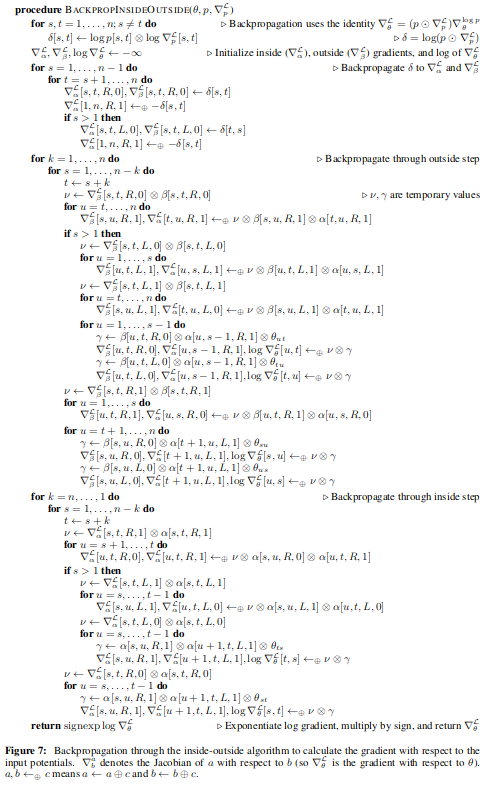
\includegraphics[height=.7\textheight]{img/backprop-inside-outside.png}}}
\end{frame}
\againframe<8-9>{mainidea}
\begin{frame}<1>[label=smapsolution]
\cornercite{sparsemap}%
\frametitle{SparseMAP solution}
\makebox[\textwidth][c] {
\renewcommand{\arraystretch}{3}
\begin{tabular}{r@{~=~}l}
    $\mg^\star$ & $\displaystyle \argmax_{\mg \in \Mp} \mg ^\top \pr - \nicefrac{1}{2} \|\mg\|^2$ \\
    &\cartoonSparse[.7] $=~.6$ \cartoon[.7]{1/4,2/5} $+~.4$
    \cartoon[.7]{1/4,1/5} %\\
%    &$\bs{A}\p^\star$ with very sparse $\p^\star \in \triangle^N$
\end{tabular}
}
\centering
{\small ($\mg^\star$ is unique, but may have multiple decompositions $\p$. Active Set
recovers a sparse one.)}
\end{frame}
%
%
\begin{frame}
%
\frametitle{Algorithms for SparseMAP}
%
\vspace{-1.5\baselineskip}
\uncover<1->{
\[\mg^\star = \argmax_{\tikzmark{constr}\mg \in \Mp} \mg ^\top \pr
 -\nicefrac{1}{2} \|\mg\|^2\tikzmark{quadr}\]}
\\[\baselineskip]
\begin{columns}%
\fontsize{12pt}{14}\selectfont%
\uncover<3->{
\begin{column}{.5\textwidth}%
\vbox to .5\textheight{%
\centering
\textbf{Conditional Gradient} \\
\citep{fw,cg}
\begin{itemize}
    \item<4-> select a new corner of $\Mp$
    \item<6-> update the (sparse) coefficients of $\p$
        \begin{itemize}
            \item<6-> Update rules: vanilla, away-step, pairwise
            \item<7-> Quadratic objective: \textbf{Active Set}\\
a.k.a.\ Min-Norm Point, \citep{mnp}\\
\citep{ad3,nocedalwright,vinyes}
%\color{mygr}{\scriptsize\parencite[][Ch.~16.4 \& 16.5]{nocedalwright}}\\
%\color{mygr}\citep[][Ch.~16.4 \& 16.5]{nocedalwright}}\\

\end{itemize}
\end{itemize}
}\end{column}}
\uncover<9->{%
\begin{column}{.5\textwidth}%
\vbox to .5\textheight{%
\centering
\textbf{Backward pass}\\[2\baselineskip]
$\frac{\partial \mg}{\partial \pr}$ is sparse\\
\uncover<10->{%
computing $\left(\frac{\partial \mg}{\partial \pr}\right)^\top \bs{d}y$ \\
takes $\mathcal{O}(\operatorname{dim}(\mg)\operatorname{nnz}(\p^\star))$}
}\end{column}}
\end{columns}
\begin{tikzpicture}[%
    remember picture,
    overlay,
    expl/.style={font=\small}]
\uncover<2->{
    \node[expl,anchor=north east] (explquadr)
        at ($(current page.north east) - (.5, 2)$)
        {quadratic objective};
    \path (explquadr.west) edge[->,very thick,bend left] ([yshift=-0.5ex]{pic cs:quadr});
}
\uncover<2->{
    \node[expl,anchor=north west,align=left] (explconstr)
        at ($(current page.north west) + (.5, -2)$)
        {linear constraints\\%
         \textcolor{mygr}{\emph{(alas, exponentially many!)}}};
    \path (explconstr.south east) edge[->,very thick,bend right] ([yshift=-1ex]{pic cs:constr});
}
\end{tikzpicture}
\uncover<5>{\overlaybox[.8]{
        $\displaystyle \argmax_{\mg \in \Mp} \mg^\top~
\underbrace{(\pr - \mg^{(t-1)})}_{\widetilde\pr}$
}}
\uncover<8>{\overlaybox{Active Set achieves \\ \textbf{finite} \&
    \textbf{linear} convergence!}}
\uncover<11>{\overlaybox[.5]{Completely modular: just add MAP}}
\end{frame}

{
\setbeamercolor{background canvas}{bg=myfg}
\setbeamercolor{normal text}{fg=mybg}
\setbeamercolor{frametitle}{fg=mybg}
\usebeamercolor[fg]{frametitle}
\usebeamercolor[fg]{normal text}
\begin{frame}[plain]%
\cornercite{esim}%
\hspace{1ex}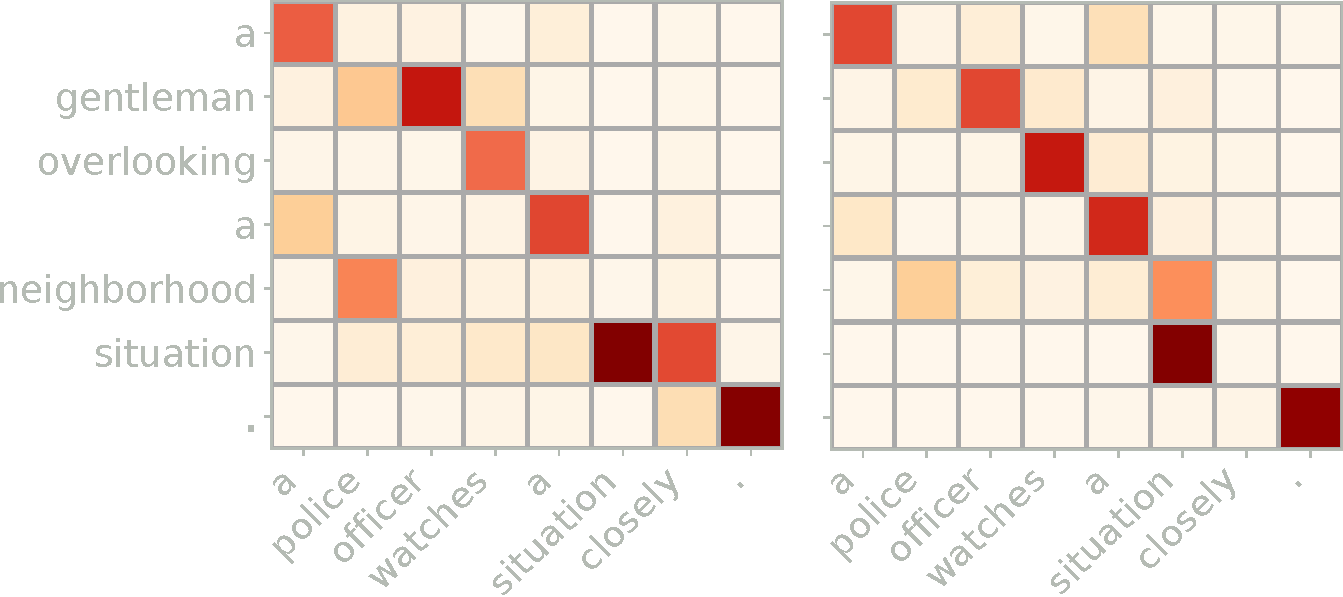
\includegraphics[height=.7\textheight]{img/snli_softmax.pdf}
\end{frame}

\newcommand*\transpmatch[3]{
\foreach[count=\i] \j in {#3}%
\draw[tPeony,thick, opacity=#1,
      {Circle[length=.6mm,width=.6mm]}-{Circle[length=.6mm, width=.6mm]}]
      ($(s\i.east) + (0, #2)$) -- ($(t\j.west) + (0, #2)$);
}
\begin{frame}[plain]%
\cornercite{sparsemap}%
\hspace{1ex}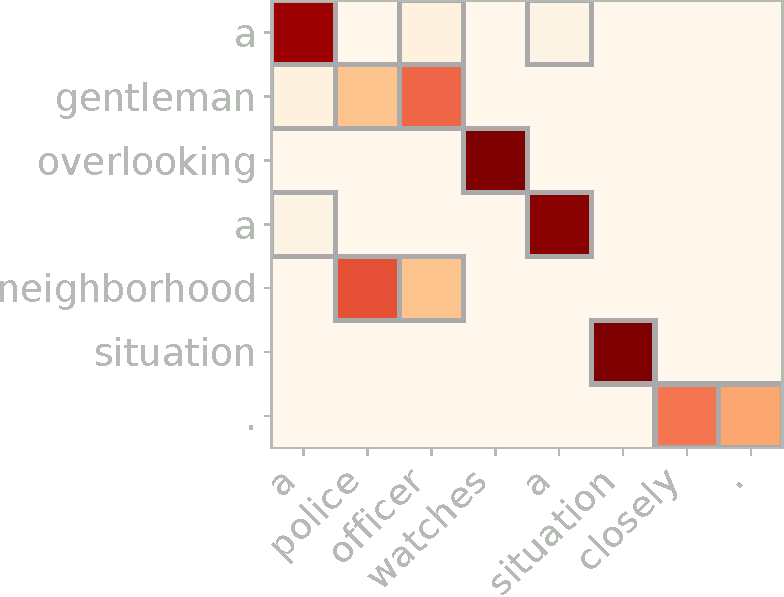
\includegraphics[height=.7\textheight]{img/snli_matching.pdf}%
%
%
\raisebox{3ex}{%
\def\xp{0}%
\def\xh{2}%
\def\baseh{0}%
\def\basep{0.3}%
\def\H{0.7}%
\footnotesize%
%
\begin{tikzpicture}%
\node[anchor=east] at (\xp, \basep+6*\H) (s1) {A};
\node[anchor=east] at (\xp, \basep+5*\H) (s2) {gentleman};
\node[anchor=east] at (\xp, \basep+4*\H) (s3) {overlooking};
\node[anchor=east] at (\xp, \basep+3*\H) (s4) {a};
\node[anchor=east] at (\xp, \basep+2*\H) (s5) {neighborhood};
\node[anchor=east] at (\xp, \basep+1*\H) (s6) {situation};
\node[anchor=east] at (\xp, \basep+0*\H) (s7) {.};
%
\node[anchor=west] at (\xh, \baseh+7*\H) (t1) {A};
\node[anchor=west] at (\xh, \baseh+6*\H) (t2) {police};
\node[anchor=west] at (\xh, \baseh+5*\H) (t3) {officer};
\node[anchor=west] at (\xh, \baseh+4*\H) (t4) {watches};
\node[anchor=west] at (\xh, \baseh+3*\H) (t5) {a};
\node[anchor=west] at (\xh, \baseh+2*\H) (t6) {situation};
\node[anchor=west] at (\xh, \baseh+1*\H) (t7) {closely};
\node[anchor=west] at (\xh, \baseh+0*\H) (t8) {.};


\transpmatch{.1}{-4pt}{5,2,4,1,3,6,8}%
\transpmatch{.2}{-2pt}{3,1,4,5,2,6,8}%
\transpmatch{.2}{-0pt}{1,3,4,5,2,6,8}%
\transpmatch{.8}{+2pt}{1,2,4,5,3,6,8}%
\transpmatch{1}{+4pt}{1,3,4,5,2,6,7}%

\end{tikzpicture}}
\end{frame}}


\againframe<4>{overview}

\begin{frame}%
\newcommand*\parcolor{myfg}
\newcommand*\clfcolor{myfg}
\newcommand*\colParseZero{mybg}
\newcommand*\colParseNonz{mybg}
\only<2->{
\renewcommand*\parcolor{tPink}
\renewcommand*\clfcolor{tDY}
}
\only<14->{
\renewcommand*\colParseZero{mybg!25!box}
\renewcommand*\colParseNonz{mybg}
}
\frametitle{Structured latent variables without sampling}
\begin{align*}
    \EE_{\z}\big[L(\z)\big] &= \tikzmark{sum}\sum_{\z \in \ZZ}
    \textcolor{\clfcolor}{L\big(\hat{y}\tikzmark{clfp}_{\uncover<2->{\clfp}}(\z)\big)}~%
    \textcolor{\parcolor}{\pi\tikzmark{parp}_{\uncover<2->{\parp}}(\z \mid x)}%
% \\
%    \uncover<3->{
%        &= \EE_{h \sim \textcolor{\parcolor}{p_{\parp}(h \mid x)}}~%
%        \textcolor{\clfcolor}{p_{\clfp}(y\mid h, x)}
%    }
\end{align*}
%\vspace{.2\baselineskip}
\vfill
\makebox[\textwidth][c]{%
\begin{minipage}{\textwidth}\centering
\par
\fontsize{12pt}{14}\selectfont%
{%
\uncover<6->{%
\textbf{How to define {\boldmath $\textcolor{\parcolor}{\pi_{\parp}}$}?}%
}
\par
\renewcommand{\arraystretch}{1.25}
\begin{tabular}{r l c c c c}
& & &
\uncover<7->{$\displaystyle \sum_{h \in \mathcal{H}}$} &
\uncover<8->{$\displaystyle \pfrac{\EE\big[L(\z)\big]}{\textcolor{\parcolor}{\parp}}$}
\\
\uncover<6->{\textcolor{mygr}{idea 1}} &
\uncover<9->{$\textcolor{\parcolor}{\pi_{\parp}(\z)}
\propto \exp \big( f_{\parp}(\z) \big) $}
& \uncover<9->{softmax}
& \uncover<11->{\emoji{oface}}
& \uncover<10->{\emoji{happ}} \\
\uncover<6->{\textcolor{mygr}{idea 2}} &
\uncover<13->{$\textcolor{\parcolor}{\pi_{\parp}(\z)} = 1$ if $\z =
\operatorname{MAP}(f_{\parp}(\cdot))$ else $0$}
& \uncover<13->{argmax}
& \uncover<14->{\emoji{happ}}
& \uncover<15->{\emoji{frown}} \\
%
\uncover<6->{\textcolor{mygr}{idea 3}} &
& \uncover<17->{SparseMAP} & \uncover<17->{\emoji{happ}} & \uncover<17->{\emoji{happ}}
\end{tabular}%
}%
\end{minipage}}

\begin{tikzpicture}[%
    remember picture,
    overlay,
    expl/.style={font=\small}]
\uncover<3->{
    \node[expl,anchor=north east] (explpar)
        at ($(current page.north east) - (.5, 1.5)$)
        {\emph{e.g.},\ a TreeLSTM defined by $\z$};
    \path (explpar.west) edge[->,very thick,bend right] ([yshift=1.5ex]{pic cs:clfp});
}
%
\uncover<5->{
    \node[expl,anchor=north west,align=left] (explsum)
        at ($(current page.north west) + (.5, -1.5)$)
        {sum over \\ all possible trees};
    \path (explsum.east) edge[->,very thick,bend left] ([yshift=2.5ex]{pic cs:sum});
}
\uncover<4->{
    \node[expl,anchor=north east,align=right] (explscore)
        at ($(current page.north east) - (.5, 4)$)
        {parsing model,\\using some scorer $f_{\parp}(\z;x)$};
    \path (explscore.west) edge[->,very thick,bend left] ([yshift=-.5ex]{pic cs:parp});
}

% HERE highlight
% \uncover<10>{%
%     \draw[
%         tBlue,
%         opacity=.5,
%         ultra thick]
%         ($(pic cs:argmax1)!.5!(pic cs:argmax2)$) ellipse (1cm and .5cm);
% }
\end{tikzpicture}%
\uncover<5>{\overlaybox[.8]{Exponentially large sum!}}
\uncover<12>{\overlaybox{All methods we've seen require sampling; hard in
general.}}
\uncover<16>{\overlaybox{STE / SPIGOT relax $\hat{y}$ in backward.}}
\end{frame}


\begin{frame}
\newcommand*\clfColor{tDY}
\frametitle{Structured latent variables without sampling}
\centering
\begin{tabular}{r@{~~}l@{\,}l@{}l@{\,}l@{\,}l@{\,}l@{\,}l}
    \miniparse{a/b/l/.7,a/c/l/1,c/b/r/.4}$ =$
    & $.7\times$ & \miniparse{a/b/l/1,a/c/l/1} & &+  $.3\times$&  \miniparse{c/b/r/1,a/c/l/1}
    & \uncover<2->{ $+ 0\times$} &
    \uncover<2->{\miniparse{a/b/l/1,b/c/l/1} + ...}
    \\
\uncover<3->{
     $\EE[L(\z)] =$ &
     $.7\times$ \textcolor{\clfColor}{$L($} &
     \miniparse{a/b/l/1,a/c/l/1} &
     \textcolor{\clfColor}{$)$}&+ $.3\times$ \textcolor{\clfColor}{$L($} &
     \miniparse{c/b/r/1,a/c/l/1} &
     \textcolor{\clfColor}{$)$}&
}
\end{tabular}
\\[2\baselineskip]
{
\small
\textcolor{mygr}{recall our shorthand}
$L(\z) = L(\hat{y}_{\clfp}(\z), y)$
}
\end{frame}
%
\begin{frame}
\cornercite{corro2019acl}
\small
\begin{columns}
\begin{column}{.4\textwidth}
\centering {Stanford Sentiment (Accuracy)} \\[1ex]
\begin{tabular}{l r}
\multicolumn{2}{l}{Socher et al} \\
Bigram Naive Bayes     & 83.1 \\[.3ex]
\multicolumn{2}{l}{\citep{sparsemapcg}} \\
TreeLSTM w/ CoreNLP    & 83.2 \\
TreeLSTM w/ SparseMAP  & 84.7 \\[.3ex]
\multicolumn{2}{l}{\citep{corro2019acl}} \\
GCN w/ CoreNLP         & 83.8 \\
GCN w/ Perturb-and-MAP & 84.6
\end{tabular}
\end{column}
\begin{column}{.6\textwidth}
\centering {Stanford Natural Language Inference (Accuracy)} \\[1ex]
\begin{tabular}{l r}
\multicolumn{2}{l}{\citep{structured_attn}} \\
Simple Attention & 86.2 \\
Structured Attention & 86.8 \\[.3ex]
\multicolumn{2}{l}{\citep{lapata}} \\
100D SAN - & 86.8 \\[.3ex]
\multicolumn{2}{l}{Yogatama et al} \\
100D RL-SPINN     & 80.5 \\[.3ex]
\multicolumn{2}{l}{\citep{choi2017learning}} \\
100D ST Gumbel-Tree & 82.6 \\
300D - & 85.6 \\
600D - & 86.0 \\[.3ex]
\multicolumn{2}{l}{\citep{corro2019acl}} \\
Latent Tree + 1 GCN - & 85.2 \\
Latent Tree + 2 GCN - & 86.2 \\[.3ex]
\end{tabular}
\end{column}
\end{columns}
\end{frame}
%
